\documentclass[hyperref,publist,addack,firstparindent]{technionThesis}
% OPTIONS: 
% hyperref          Add hyperlinks
% publist           Add a list of publications in the front pages (update list in thesissetup.sty)
% addack            Add an acknowledgments page (only for final version!)
% advisement        Use `advisement' instead of `supervision' in front pages 
% spacepar          Add a blank line between paragraphs
% firstparindent    Indent the first paragraph of a chapter/section
% libertine         Use libertine as the main document font rather than computer modern roman

% Define your own data in the following file
\usepackage{technionThesisSetup}

% Use the following file to define your own macros
\usepackage{technionThesisMacros} 

% For generating dummy text. Remove from your version.
\usepackage{lipsum}


\begin{document}
% FRONT PAGES:
\makeTitleEnglish

\chapter{Abstract}
This work proposes an algorithm for finding sparse vertex to vertex correspondences between shapes in three dimensions. The method is designed to address three challenging cases: large non rigid deformations, partiality of the shapes, and topological noise. 
At the core of the method lies a novel, yet simple, similarity measure that analyzes statistical properties of the nearest-neighbor field, which is a mapping of vertices in a local shape descriptor space from the source surface to their nearest neighbors on the target shape. This information is shown to be powerful, compared to minimizing some function of distances. In particular, our proposed similarity function analyzes the diversity of the nearest-neighbor field and its preservation of distances. 
Our algorithm leverages the proposed similarity measure with respect to smaller sub surfaces at multiple sizes, in order to obtain a sparse, yet coherent set of vertex to vertex correspondences,. The latter can then be turned into dense correspondences using existing methods. 
We provide an extensive empirical evaluation of our algorithm on existing common shape correspondence benchmarks. We show that our method outperforms  existing state-of-the-art methods. In particular,  the results on partial matching benchmarks shows that our method outperforms the best existing techniques, both quantitatively and qualitatively by a significant margin. \clearpage
\section*{Abbreviations}
\begin{longtable}[l]{ll}
    A1  & An abbrevation \\ 
    A2  & Another abbrevation 
\end{longtable}
% NOTE: The list of abbreviations may exceed one page. The longtable environvment takes care of this. 
   \cleardoublepage

% Each of the following should begin with \chapter{...}. 
\chapter{Introduction}\label{chap:intro}
% {First paragraph: problem definition + applications
\begin{figure*}[b!]
	\centering
	\setlength\tabcolsep{3pt}
	\begin{tabular}{ccc}
		%	\rotatebox{90}{    \, FAUST} &
		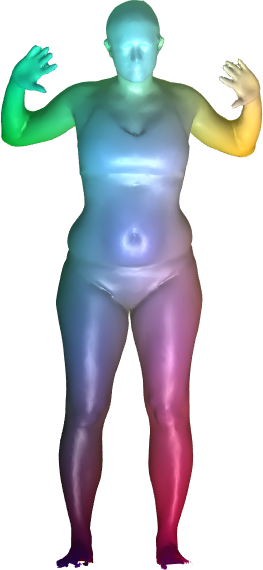
\includegraphics[width=0.1\textwidth]{figures/test_scan_031_test_scan_034_PFM.png}  &
		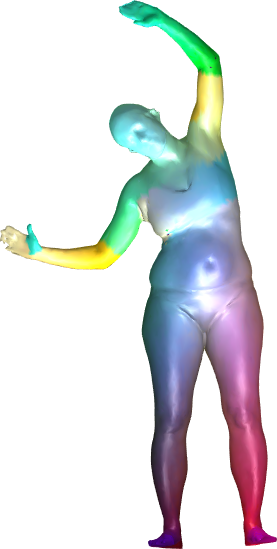
\includegraphics[width=0.1333\textwidth]{figures/test_scan_034.png} &
		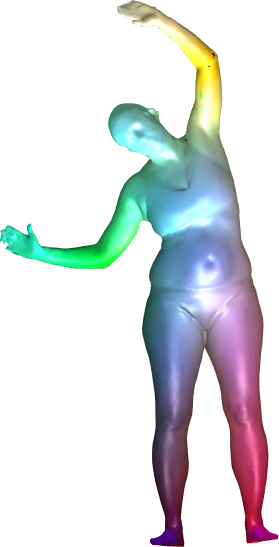
\includegraphics[width=0.1333\textwidth]{figures/test_scan_031_test_scan_034.png}\\
		\multicolumn{3}{c}{(a) large deformations}\\
		%	 \rotatebox{90}{    \, SHREC'16A} &
		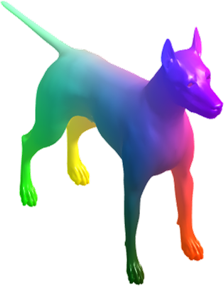
\includegraphics[scale=0.5]{figures/dog_base.png}&
		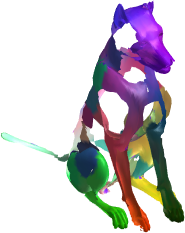
\includegraphics[scale=0.55]{figures/holes_dog_shape_25_PFM.png}&
		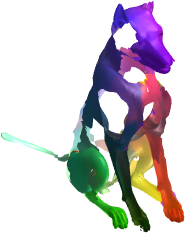
\includegraphics[scale=0.55]{figures/holes_dog_shape_25.png}\\
		\multicolumn{3}{c}{(b) partiality}\\
		%	\rotatebox{90}{    \, SHREC'16B} &
		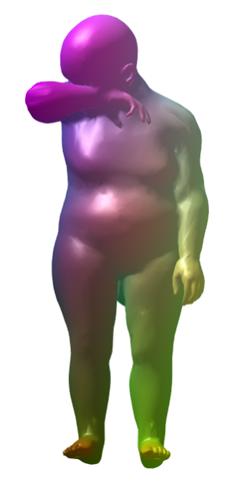
\includegraphics[width=0.12\textwidth]{figures/Top1Base.png} &
		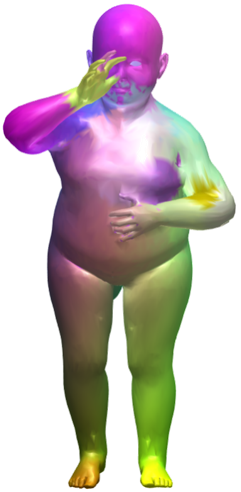
\includegraphics[width=0.12\textwidth]{figures/Top1PFM.png} &
		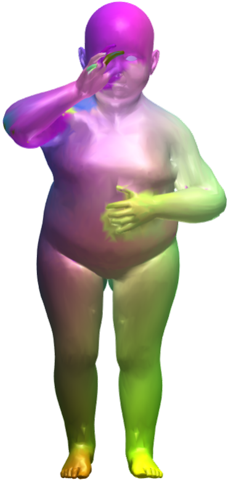
\includegraphics[width=0.12\textwidth]{figures/Top1DDIS.png} \\
		\multicolumn{3}{c}{(b) topological noise}\\\\
		Input & Rodola'17\cite{rodola2017partial} & Ours \\
	\end{tabular}
	\caption{{\textbf{Challenging correspondences.}}  
		Corresponding vertices are colored similarly.
		(a) While the corresponding arms are switched in~\cite{rodola2017partial}, our algorithm manages to match the arms correctly.
		(b) When given a highly partial model of a dog as input, our algorithm manages to match its four dog's legs correctly.
		(c) The right hand is well matched by our algorithm. 
	}
	\label{fig:teaser}
\end{figure*}

Shape correspondence is a fundamental problem in computer vision and computer graphics, both in 2D and in 3D.
Numerous applications require robust correspondences, for instance in animation, reconstruction, and shape analysis~\cite{van2011survey}.
The focus of this paper is on shape correspondence between meshes in 3D.




Finding correspondences between shapes is highly challenging, even when the objects are rigid and full~\cite{Biasotti03,barequet1997partial,mellado2014super,Zeng_2017_CVPR}. 
This paper, however, addresses the problem of shape correspondence, when the following additional challenges are added (see Figure~\ref{fig:teaser}):
(1)~The objects may have gone through non-rigid deformations~\cite{dubrovina2010matching,lipman2009mobius,Maron:2016:PRV:2897824.2925913,solomon2016entropic,vestner2017product}; 
(2)~only part of the shape is given and should be  matched to the correct region within the full shape ({\em partiality})~\cite{biasotti2006sub,itskovich2011surface,rodola2017partial,sahilliouglu2012minimum},  and
(3)~non-adjacent parts of the surfaces intersect~\cite{chen2015robust,litany2017fully,vanKaick:2013:BMP:2771539.2771553,vestner2017efficient} ({\em topological noise}).
All of the above frequently occur in real world scenarios.

% second paragraph: related work in short
Previous approaches have focused on minimization of some distortion criteria, of either point-wise shape descriptors~\cite{litany2017fully,rodola2017partial}, pair-wise shape descriptors~\cite{sahilliouglu2012minimum}, or the combination of both~\cite{vestner2017efficient}.
Impressive result have been exhibited , yet some downfalls still exist.
This is in particular evident in the three cases mentioned above, in particular when the  deformation is extreme, when partiality is severe, and in many cases of topological noise.

Some recent approaches have utilized deep neural networks~\cite{boscaini2016learning,litany2017deep,Masci:2015:GCN:2919341.2920992,monti2017geometric}.
These show a lot of promise on a couple of full-shape benchmarks. 
In~\cite{boscaini2016learning} the results are analyzed also for a  partial correspondence benchmark; 
we will show that our method outperforms their results.
All these methods require a significant amount of labeled training data, which is currently difficult to acquire. 

The algorithm proposed in this paper belongs to the first class of algorithms, which does not utilize deep learning.
It proposes a novel similarity function, which analyzes the nearest neighbor field in vertex shape descriptor space.
That is to say, for each vertex of a source mesh we find the nearest neighbor in the target mesh, in terms of a specific shape descriptor and a distance function.
Rather than minimizing some function of distances, we analyze statistics of this field.
The statistical nature of our method lets it ignore outliers, which are the source of unreliability in some other methods.
Specifically, the statistics we are concerned about regard two aspects of the nearest neighbor field:
(1) the diversity of the field, i.e. how many different matches the nearest neighbor field contains, and
(2) preservation of pairwise distances of the matches in the nearest neighbor field.

We have tested our method on the two challenging benchmarks of {\em SHREC'16}, the one that contains partial deformed shapes~\cite{cosmo2016shrec} and and the one that contains deformed shapes with topological noise~\cite{lahner2016shrec}.
We exhibit the benefit of our method both qualitatively (Figure~\ref{fig:teaser}) and quantitatively.
In particular, our method obtains a $10$-$20\%$ improvement over the state-of-the-art on the first dataset and is competitive on the second.
In addition, we also show qualitative results on the FAUST dataset~\cite{bogo2014faust}.

Hence, our contribution is twofold.
\begin{enumerate}
	\item
	We introduce a new approach for finding correspondences between given meshes, which is robust to deformations, partiality and topological noise.
	The novelty of our approach is relying on properties of the nearest-neighbor field.
	\item
	We demonstrate the benefits of our algorithm on the commonly-used benchmarks, both quantitatively and qualitatively.
\end{enumerate}

\chapter{Related work}\label{chap:related work}

%%%%%%%%%%%%%%%%%%%%%%%%%%%% Matching Of Deformable Surfaces
\paragraph{Correspondence of deformable shapes in 3D}
The problem of finding shape correspondences between deformable objects in 3D has been studied extensively.
Most methods attempt to minimize some distortion criteria, which falls into one of three categories:
(1)~local shape similarity, commonly computed as the distance between corresponding point descriptors~\cite{aubry2011wave,bronstein2010scale,jain2007non,rusu2008learning,rusu2009fast,Sun:2009:CPI:1735603.1735621,tombari2010unique,dey2010persistent}, 
(2)~pairwise relations~\cite{chen2015robust,coifman2005geometric,vestner2017product}, or
(3)~a combination of both~\cite{vestner2017efficient}.

%Partial Matching Of Deformable Surfaces
The underlying assumption of most of these methods is that the shapes are either approximately isometric or that they are topologically homeomorphic.
This assumption usually do not hold in the case of partial correspondence and topological noise.

A variety of approaches have been proposed to handle topological differences.
In~\cite{ovsjanikov2008global}, resilience to topological shortcuts in the context of intrinsic
symmetry detection of deformable shapes is studied.
Wang et al.~\cite{wang2011discrete} considered the metrics induced by commute-time kernels as a more robust alternative to geodesic distance.
In~\cite{rodola2013elastic,Torsello:2012:GAD:2354409.2354702} sparse relaxations to this framework were introduced.
A different kernel was proposed by~\cite{boscaini2014coulomb} and bilateral maps were suggested by~\cite{vanKaick:2013:BMP:2771539.2771553}.
Chen and Koltun~\cite{chen2015robust} reformulated the isometric embedding problem with a robust norm accounting for topological artifacts.
Boscaini et al.~\cite{Boscaini2016AnisotropicDD} proposed a CNN-based shape descriptor to address the problem.
Litani et al.~\cite{litany2017fully} modified the functional mapping of~\cite{Ovsjanikov:2012:FMF:2185520.2185526} to better handle topological noise.
Vestner et al.~\cite{vestner2017efficient} formulated the problem as a quadratic assignment problem that incorporates matching of both point-wise and pair-wise descriptors.

Partial correspondence was first tackled, assuming that the shapes are rigid~\cite{Aiger:2008:CSR:1360612.1360684,albarelli2015fast,itskovich2011surface}.
In the non-rigid case, the notion of  minimum distortion correspondence was utilized~\cite{bronstein2009partial,rodola2013elastic,Torsello:2012:GAD:2354409.2354702}.
A voting-based method was proposed by~\cite{sahilliouglu2014multiple}, to match shape extremities.
Other works include the alignment of tangent spaces~\cite{Brunton:2014:LRR:2592295.2592390} and the design of robust descriptors for partial matching~\cite{vanKaick:2013:BMP:2771539.2771553}.
In the context of collections of shapes, partial correspondence has been considered in~\cite{cosmo2017consistent,huang2014functional}.
Masci et al.~\cite{Masci:2015:GCN:2919341.2920992} introduced a deep learning framework for computing a dense correspondence between deformable shapes.
\cite{boscaini2016learning}~improved upon this by introducing anisotropic convolution kernels.
In~\cite{rodola2017partial,litany2017fully} the notion of functional maps~\cite{Ovsjanikov:2012:FMF:2185520.2185526} was adapted to the partial matching scenario.

The method introduced in this paper addresses both partial matching and topological noise.
We present a novel similarity measure that inherently differs from the above methods.
Instead of relying explicitly on distances between descriptors, our similarity measure is based on statistics of simple properties of the nearest neighbor field between the points of the two given surfaces.

%%%%%%%%%%%%%%%%%%%%%%%%%%%%%%%% section: 2D Shape Matching
\paragraph{Correspondence of deformable shapes in images}
% copy from Roey
In images, partial matching is often termed {\em template matching}.
Numerous papers have attempted to solve the problem; a good review is given in~\cite{ouyang2012performance}.
The commonly-used methods are pixel-wise~\cite{chen2003fast,hel2014matching}.
Geometric transformations have also been addressed~\cite{tian2012globally,tsai2002rotation}.
Another group of methods considers a global probabilistic property of the template~\cite{comaniciu2000real,oron2015locally}.
Recently, machine learning based techniques have also been used~\cite{aberman2018neural}.

Our work is inspired by the methods of~\cite{dekel2015best,talmi2017template}, which also look at various statistics of the nearest-neighbor field of the correspondence.
In particular, in~\cite{dekel2015best} it is proposed to simply count points which are mutually nearest neighbors of each other.
In~\cite{talmi2017template} it is suggested to rely mostly on a subset of matches---on points that have distinct nearest neighbors.
We adopt this general approach, but use other criteria, which are more suitable to surfaces in 3D that are orderless and lack constant density.
\chapter{Another  Chapter}\label{chap_second}

\section{First Section}
This section has a theorem with its proof. 
It is closely related to \Cref{thm:earth} from \Cref{chap_first}. 

\begin{theorem}\label{thm:earth second}
    The Earth is not flat.
\end{theorem}

\begin{IEEEproof}
    Trivial.
\end{IEEEproof}

It also has a corollary.

\begin{corollary}
    The Earth is round.
\end{corollary}

\begin{IEEEproof}
    Follows from \Cref{thm:earth second}.
\end{IEEEproof}
Note (again) the use of the cleveref package here. 

\section{Second Section}
This section has a remark.
\begin{remark}
    Roses are red. See \Cref{lem:roses} for an explanation. 
\end{remark}

\lipsum[5-9]



% Add more chapters as required. 
% In a thesis, there must be a discussion/conclusions section
\chapter{Conclusions}\label{chap:Conclusions}

%%%%%%%%%%%%%%%%%%%%%%%%%%%%%%%%%%%%%%%%%%
%%%%%%%  section: Conclusion
%%%%%%%%%%%%%%%%%%%%%%%%%%%%%%%%%%%%%%%%%%
This paper has introduced a novel approach for finding correspondences between shapes in 3D.
This approach is based on a simple observation:
Statistical properties the nearest-neighbor field from the source surface to the target provide robust information about the correspondence.
In particular, we use the diversity of the nearest-neighbor field and the consistency of the internal distances within the surface of corresponding points. 
Two additional ideas of our approach are the use of small sub-surfaces when computing the similarity (rather than using the whole surface) and utilizing a multi-scale approach.

Our approach improves the state-of-the-art results both quantitatively and qualitatively on the challenging benchmarks of SHREC'16.
In particular, these benchmarks contain examples having large deformations, symmetries, partiality of the shapes, and topological noise.
We have demonstrated that our method is robust to the scale of partiality, as well as to its own parameters.

% An appendix must appear AFTER the discussion. 
\begin{appendices} % Set appendix numbering
    \chapter{Appendices}

\section{Appendices for Chapter~\ref{chap_first}}
\subsection{ A lovely subsection}
\lipsum[20-21]
\subsection{ Another lovely subsection}
\lipsum[21-22]

\section{Appendices for Chapter~\ref{chap_second}}
\subsection{Yet another lovely subsection}
\lipsum[23-24]
\subsection{Still a lovely subsection}
\lipsum[25-26]

\end{appendices}


% Setup the bibliography
\bstctlcite{BIBctrl}
\bibliographystyle{IEEEtranS} 
\bibliography{mybib.bib} 
\clearpage

% HEBREW SECTION
\makeTitleHebrew
\end{document}
